\chapter{The International Linear Collider}
\label{ILC}
The International Linear Collider (ILC) is a linear \electron \positron accelerator with an center-of-mass energy of \unit{500}{GeV} in the first stage and \unit{1}{TeV} in the second.
The state of the art technologies for both, the detectors and the machine, and the machine design make a clean environment and high precision measurements possible, because of which the ILC will be a unique machine.\\
The following sections will talk about the ILC layout, its possible sites, the two detectors, and finally the physics motivation for such a capable accelerator.
\section{Layout}
\label{ILC:layout}

Figure~\ref{fig:ILC_Layout} shows the schematic layout of the ILC for the \unit{500}{GeV} stage.
\begin{figure}
\centering
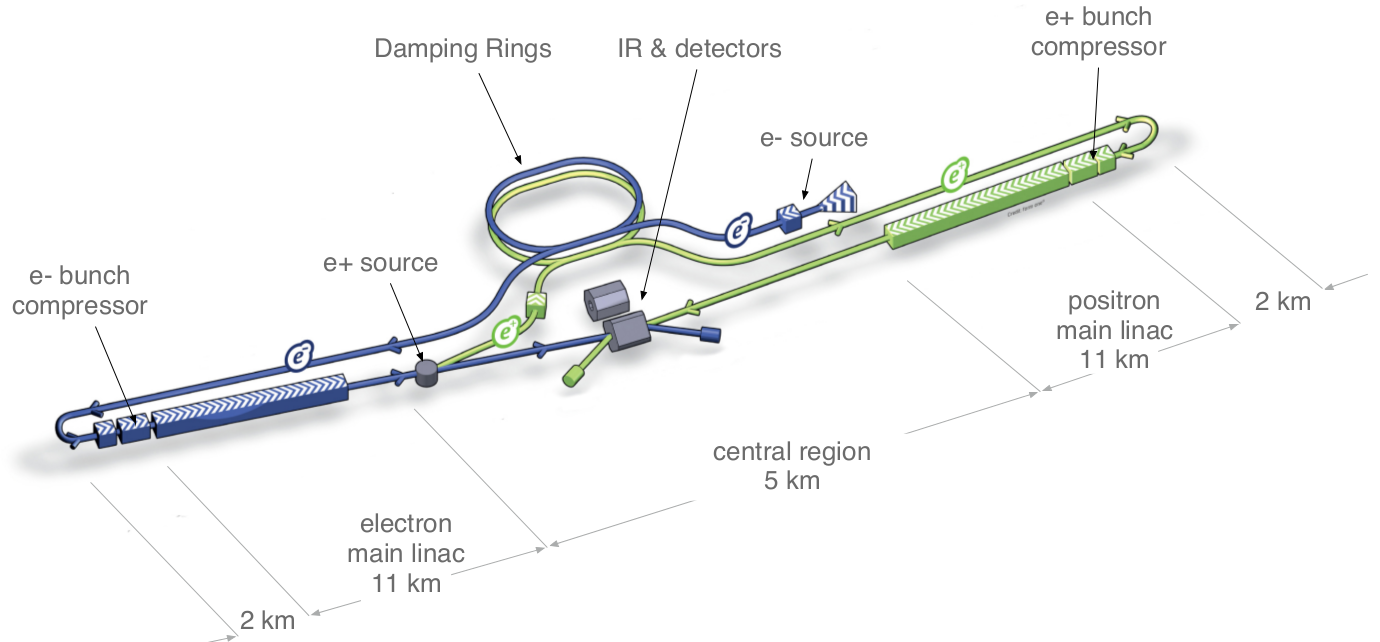
\includegraphics[width=0.8\textwidth]{Figures/ILC_layout.png}
\caption[Schematic layout of the ILC]{Schematic layout of the ILC~\cite[p. 9]{TDR1}}
\label{fig:ILC_Layout}
\end{figure}

The electrons originate in the polarized source based on a photocathode DC gun.
When these electrons pass through an undulator, high-energy photons are produced which are then converted to electron-positron pairs.
The polarized positrons from these pairs continue in the positron line which is from that point on equivalent to the electron line.
After passing the \unit{5}{GeV} Damping Rings (DR) with a circumference of \unit{3.2}{km}, the electron and positron beams are compressed into bunches by a two-stage compressor system.
Subsequent to that, the bunches are injected into the main linacs.
The main linacs have a length of \unit{11}{km}, and use superconducting radio frequency (RF) cavities with a frequency of \unit{1.3}{GHz} and an average accelerating gradient of \unit{31.5}{MV/m}.
For the machine upgrade to \unit{1}{TeV}, the linacs can be extended in length.
The Beam Delivery System (BDS), which has an overall length of about \unit{4.4}{km}, transports the bunches from the linacs to the Interaction Point (IP).
In the BDS, the beams are focused to nanometer size by the Final Focus (FF) system.
After that, the beams are then finally brought into collision with a crossing angle of \unit{14}{mrad} at the IP.\cite[p. 9-10]{TDR1}
Table~\ref{tab:ILC_parameters} shows the machine parameters for the baseline design at \unit{500}{GeV} center-of-mass energy, and for the luminosity and the energy upgrade stages.

\begin{table}
\caption{Beam parameters for different phases in the ILC operation scenario (Baseline 500, Luminosity Upgrade, TeV Upgrade)~\cite{SiDBkgNote}}.
\label{tab:ILC_parameters}
\centering
\begin{tabularx}{0.74\textwidth}{ll|rrr}
\hline\hline
& & \textbf{Baseline 500} & \textbf{Lumi Upgrade} & \textbf{TeV Upgrade}\\
\hline
\cline{1-5}
\hline
E$_{CM}$  &(\si{\GeV}) & 500  & 500  & \num{1000} \\
n$_b$ & & \num{1312} & \num{2625} & \num{2450}  \\
$\Delta t_b$ &(\si{\nano\second}) & 554  & 366   & 366 \\
N & & \num{2.0e10}  & \num{2.0e10}  & \num{1.74e10}  \\
q$_b$ &(\si{\nano\coulomb}) & 3.2  & 3.2  &  2.7  \\
$\sigma_x^*$ &(\si{\nano\metre}) & 474  & 474  &  481 \\
$\sigma_y^*$ &(\si{\nano\metre}) & 5.9 &  5.9  &  2.8 \\
$\sigma_z$ &(\si{\milli\metre}) & 0.3  &  0.3  &  0.25 \\
L &(\si{\per\centi\metre\squared\per\second}) & \num{1.8e34} & \num{3.6e34} & \num{3.6e34} \\
\hline\hline
\end{tabularx}
\end{table}

The Interaction Region (IR) houses the two detectors for the ILC, the Silicon Detector (SiD) and the International Large Detector (ILD), which are in a push-pull system.
The detectors and the push-pull system are explained in more detail in Section~\ref{ILC:detectors}.

\section{Possible Site}
\label{ILC:site}
Out of originally 10 potential ILC sites in Japan, the Kitakami mountains in the Tohuku Prefecture was chosen to be the preferred site for the ILC.
This decision was made in July 2013 after a detailed study of all site specific factors, like the geological conditions, the infrastructure, and the impact on the environment and the economy.
As can be seen in Figure~\ref{fig:ILC_Site}, the closest city with about 120,000 citizens would be Ichinoseki.
Morioka and Sendai are the biggest cities around the candidate site, with Tokyo being about \unit{430}{km} away.
Although being in the north of Japan, the travel time from Tokyo is only about three hours, and the proximity to the coast line allows the transportation of construction, machine and detector parts by ship.

\begin{figure}
\centering
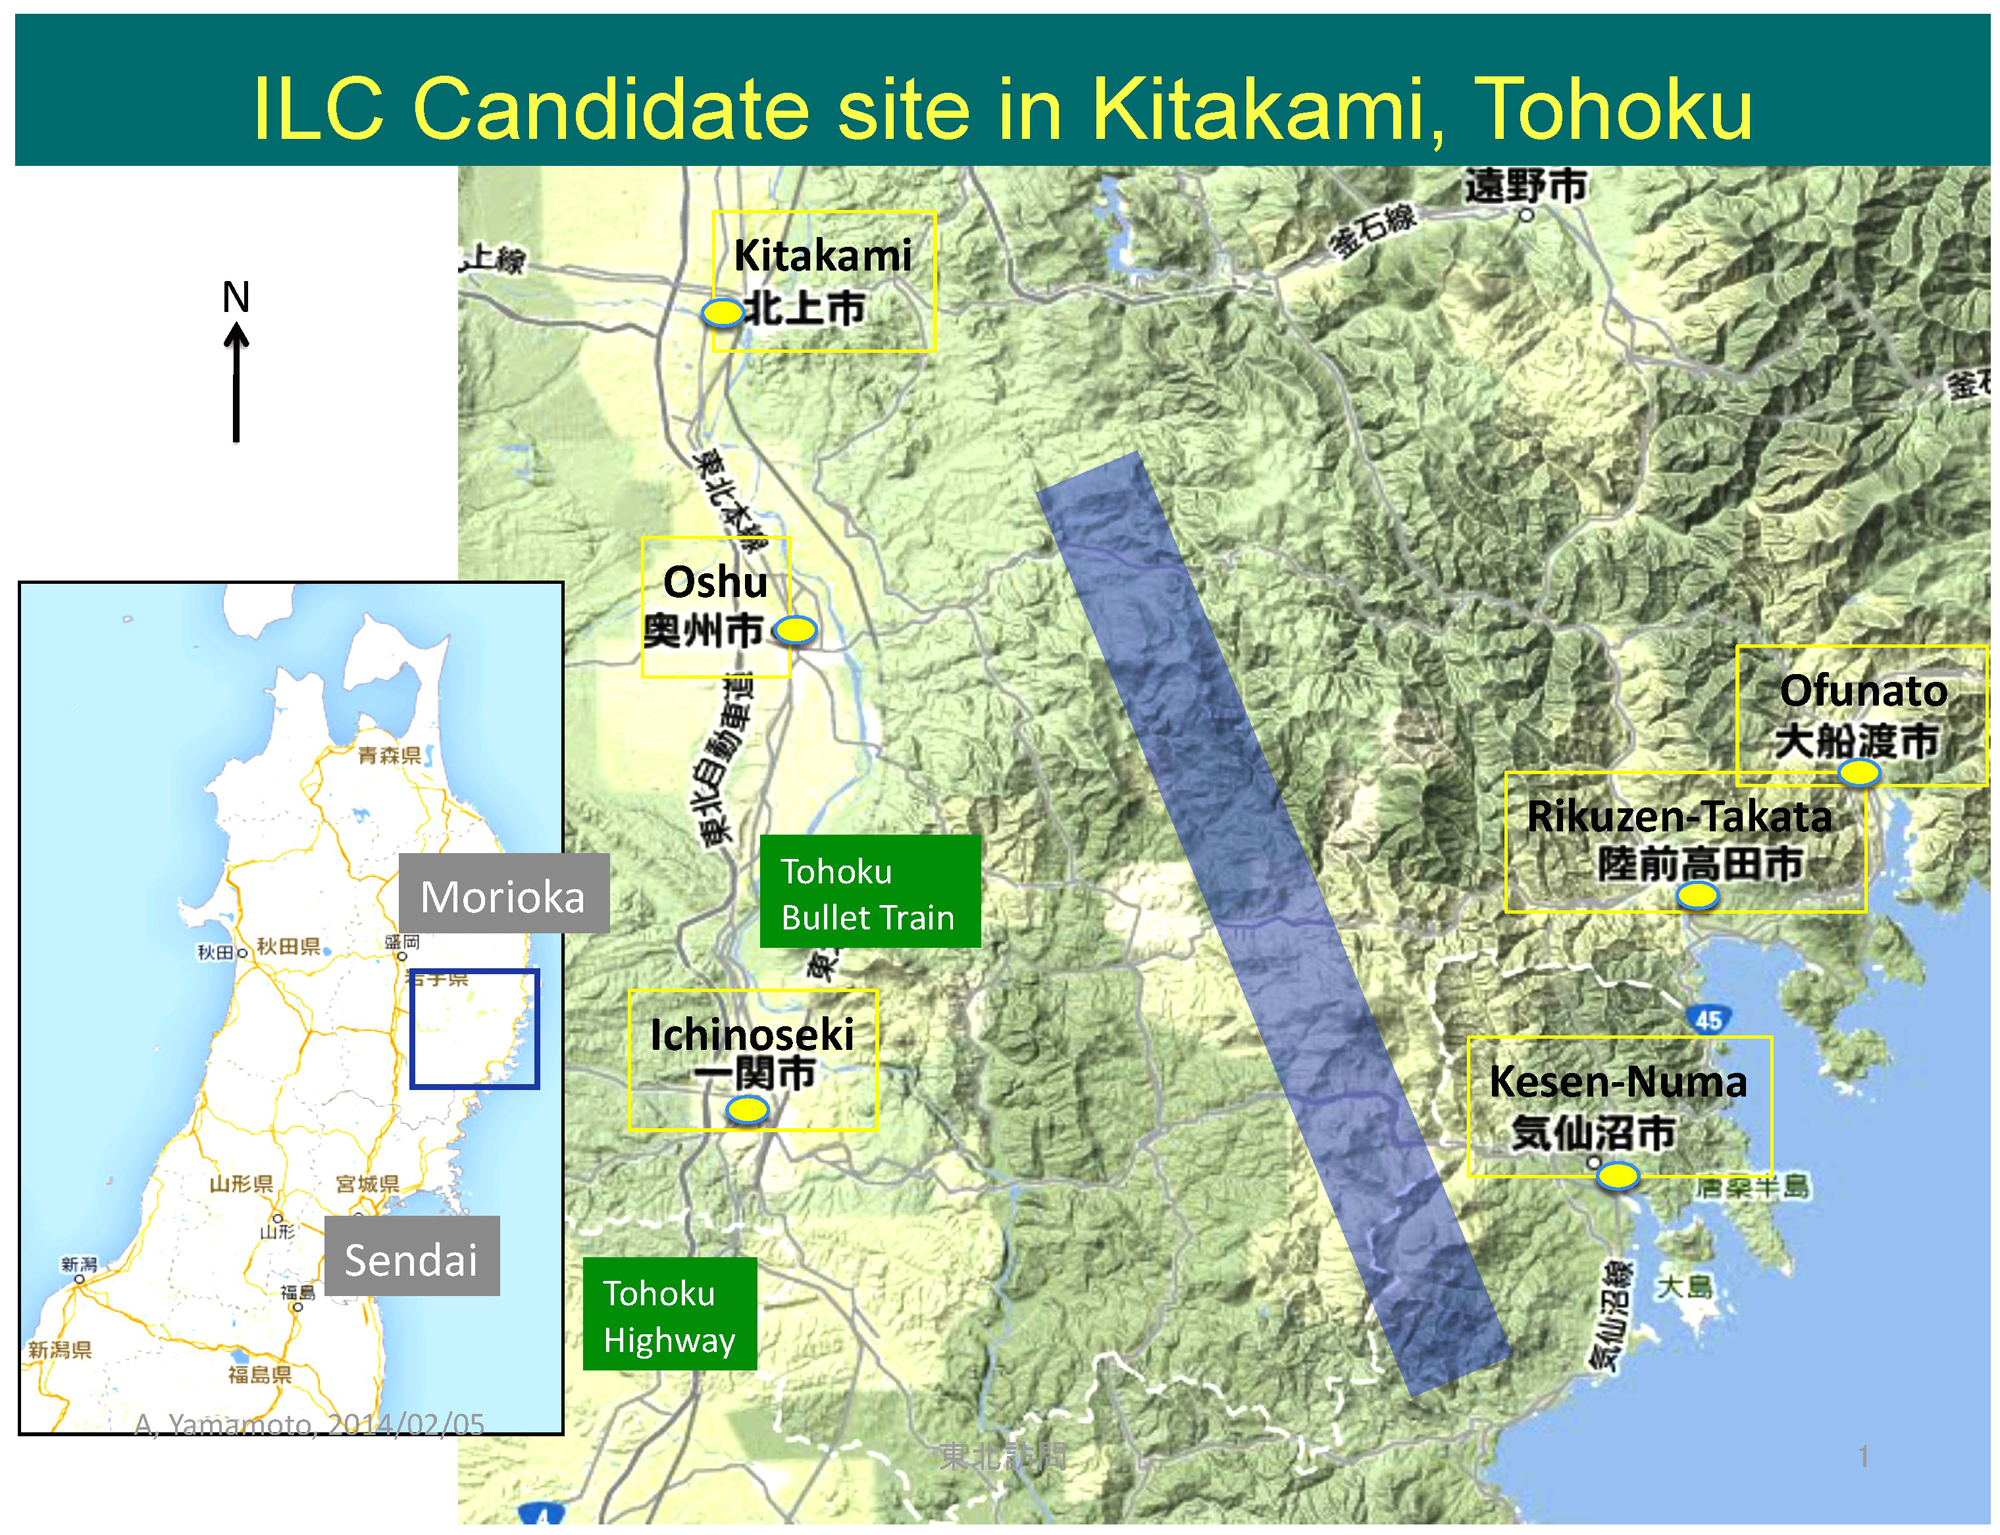
\includegraphics[width=0.6\textwidth]{Figures/ILC-site.jpg}
\caption[Possible site for the ILC]{The possible site for the ILC are the Kitakami mountains in the Tohuku Prefecture.\cite{Site}}
\label{fig:ILC_Site}
\end{figure}

\section{SiD and ILD}
\label{ILC:detectors}

In order to preserve the competitive spirit and the ability to cross-check results, the ILC has two detectors despite the fact that it is a linear and not a circular collider.
The so-called push-pull system makes that possible by allowing the detectors to switch position after a certain amount of data-taking time.
The whole detector together with the last quadrupole magnet of the accelerator Final Focus system will be pulled out of the beam line, and the other one will be pushed in.
The whole process is designed to take only a short time, i.e. several hours up to 1-2 days, but involves some challenges especially for the magnets, the cryogenics and the detector and machine alignment.\cite[p. 28-29]{TDR1}


\section{Physics Motivation}
\label{ILC:physicsmotivation}
